\documentclass[border=10pt]{standalone}
\usepackage{pgfplots}
\pgfplotsset{compat=1.18}

\begin{document}
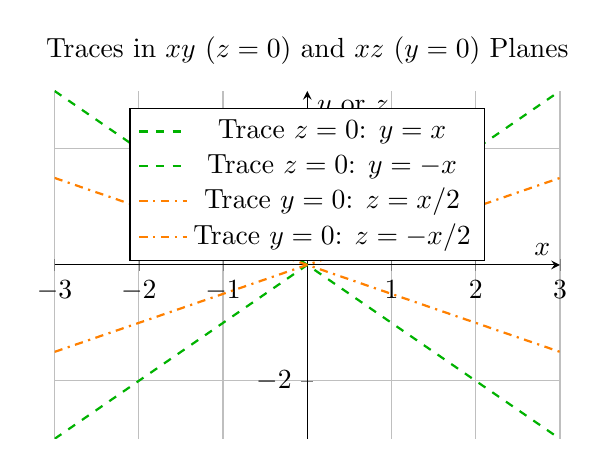
\begin{tikzpicture}
\begin{axis}[
    xlabel=$x$,
    ylabel={$y$ or $z$},
    title={Traces in $xy$ ($z=0$) and $xz$ ($y=0$) Planes},
    axis lines=center,
    domain=-3:3,
    samples=100,
    grid=major,
    width=8cm,
    height=6cm,
    legend style={at={(0.5,0.95)}, anchor=north},
    ymin=-3, ymax=3,
]

% Trace z=0: y = x
\addplot+[green!70!black, thick, dashed, no marks] {x};
\addlegendentry{Trace $z=0$: $y=x$}

% Trace z=0: y = -x
\addplot+[green!70!black, thick, dashed, no marks] {-x};
\addlegendentry{Trace $z=0$: $y=-x$}

% Trace y=0: z = x/2
\addplot+[orange, thick, dashdotted, no marks] {0.5*x};
\addlegendentry{Trace $y=0$: $z=x/2$}

% Trace y=0: z = -x/2
\addplot+[orange, thick, dashdotted, no marks] {-0.5*x};
\addlegendentry{Trace $y=0$: $z=-x/2$}

\end{axis}
\end{tikzpicture}

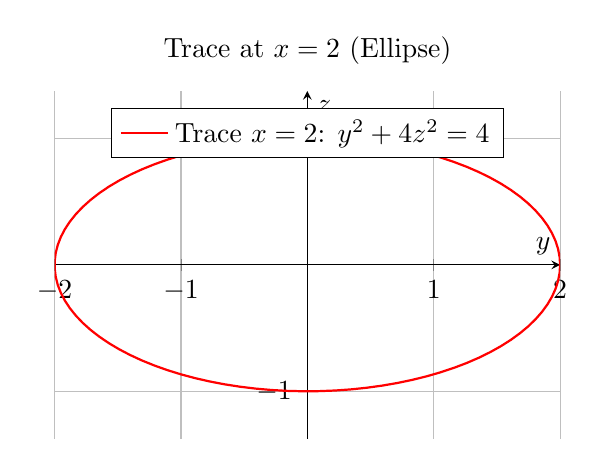
\begin{tikzpicture}
\begin{axis}[
    xlabel=$y$,
    ylabel=$z$,
    title={Trace at $x=2$ (Ellipse)},
    axis lines=center,
    domain=0:360,
    samples=100,
    grid=major,
    width=8cm,
    height=6cm,
    legend style={at={(0.5,0.95)}, anchor=north},
    axis equal,
]

% Trace x=2: y^2 + 4z^2 = 4 => y = 2cos(t), z = sin(t)
\addplot+[red, thick, no marks] ({2*cos(x)}, {sin(x)});
\addlegendentry{Trace $x=2$: $y^2 + 4z^2 = 4$}

\end{axis}
\end{tikzpicture}
\end{document}